\subsection{A Summary of Methods Previously Explored in Literature}
The table that follows summarises the methods used in literature and a brief list of advantages and disadvantages. An in-depth exploration of the papers used can be found in section \ref{subsec:in_depth_findings} and an exploration of each possible method and their suitability for this project can be found in section \ref{sec:method_exploration}.
%TC:ignore
\begin{longtabu} to \textwidth {|X[0.5]|X|X|}
\hline

	Method & Advantages & Disadvantages\\
	\hline
	\endfirsthead
	\hline
	Method & Advantages & Disadvantages \\
	\hline 
	\endhead
	\hline
	\endfoot
	Raw signal & The most accurate method of simulation available as it uses the characteristics of the radar beam in order to simulate the responses of the structures it reflects off. & Most computationally complex method as it has to simulate the effects of every beam every time a pulse is transmitted and received. \\
	Rasterisation & The fastest method of simulating SAR as it uses image transformation techniques in order to give a good idea of how an image will look, this method is capable of real-time updates of the image which means it has applications in SAR data capture planning. & The least accurate method as it is only performing an image transform as opposed to a full simulation of the signal. \\
	Ray tracing & A good balance of speed and accuracy, uses advanced computer graphics techniques to only simulate the parts of the model available to the observer so is less computationally intense than the raw signal but also more accurate than rasterisation. & Requires a good graphics processor as well as a good modelling environment in which to perform it, this is by far the most complex to implement from scratch \\
	Hybrid methods & Has the potential to be a good balance between the raw signal and ray tracing as it uses raw signal for the higher order contributions and ray tracing for the more obvious single reflections & This is the least explored method so very few conclusions about its actual performance can be drawn, with only one paper found that uses it. \\
	
\end{longtabu}
%TC:endignore
\subsection{In-Depth Findings}
\label{subsec:in_depth_findings}
\subsubsection{Raw SAR Simulation}
There are three main methods that have previously been explored for simulating SAR. The first of these, which is the most accurate is simulating the effects of the beam itself, as detailed in Franceschetti \textit{et al.} 2003 \cite{franceschettiSARRawSignal2003}. This describes creating the raw data as would be expected in a SAR system in the real world and then transforming it to create a SAR image. The ground work for this was laid in Franceschetti \textit{et al.} 1992 \cite{franceschettiSARASSyntheticAperture1992}, which itself builds on Francescetti and Schirinzi's work on a SAR processor based on two-dimensional FFT codes \cite{franceschettiSARProcessorBased1990}. This approach has the advantages of being able to take into account backscattering as well as the higher-order signal contributions created by scattering as the signal reflects off of both a wall and the ground. A lot of the preliminary work with regards to the behaviour of electromagnetic backscattering was conducted in \cite{franceschettiCanonicalProblemElectromagnetic2002}. This describes a model that allows for the return from a structure to a microwave sensor to be analysed and so determine its dielectric properties as well as its geometric properties. The optics can be altered to simulate the roughness of the surface the signal is reflected off of last before it is received by the sensor. This can also be expanded to simulate backscattering. This simulator as a whole works very well with individual objects, however the simulation time was found to scale linearly with the number of objects present in the scene. Simulations in \cite{franceschettiSARRawSignal2003} were carried out using a Pentium IV processor from Intel Corp, released in 2001 which means that the simulation times achieved are not necessarily reflective of the performance achievable on more modern processors, however at the time it was found that while one object in a 512x512 pixel image required approximately 34 seconds, two objects in the same sized image required 1'02" and 16 objects increased this computation time up to 7'38". This is not ideal if the aim is real-time or even near real-time simulation capabilities as most urban environments that are to be simulated will contain far more than 16 structures. This efficiency does seem to have been improved in Franceschetti \textit{et al.} 2007 \cite{franceschettiSimulationToolsInterpretation2007} as in this paper it is used to simulate a SAR image of a $400\times 600 \textrm{m}^2$ area of the centre of Munich, incorporating the Technische Universität and the Alta Pinakothek, which leads to a reasonably complicated scene.  \par 
\begin{figure}
\centering
\begin{subfigure}{.5\textwidth}
	\centering
	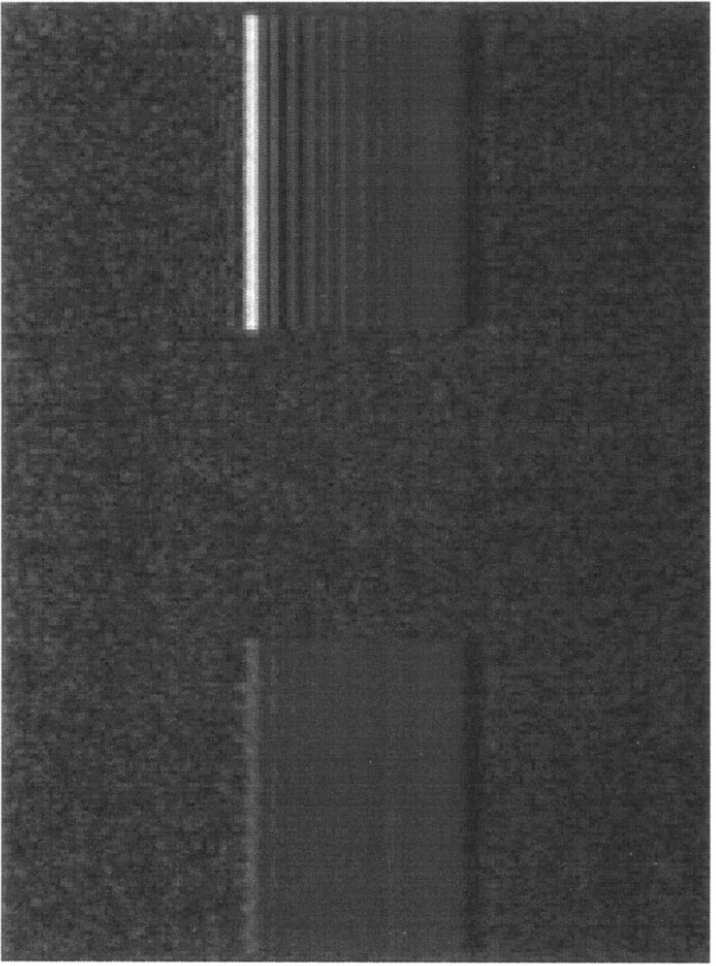
\includegraphics[width=0.9\linewidth]{../figures/franceschetti_2003_2_buildings}
	\caption{Simulated single-look SAR with two buildings}
	\label{fig:franceschetti_2003_2_buildings}
\end{subfigure}%
\begin{subfigure}{.5\textwidth}
	\centering
	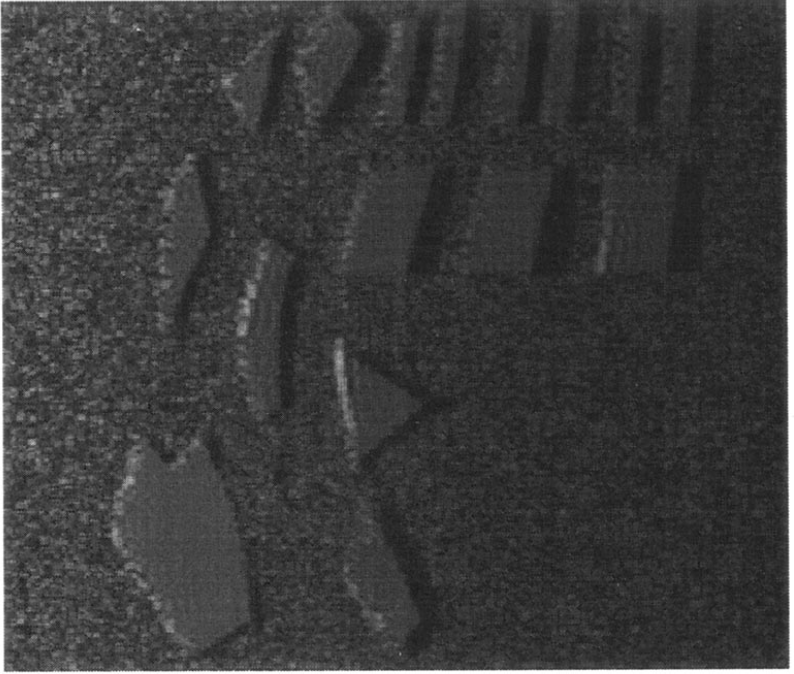
\includegraphics[width=0.9\linewidth]{../figures/franceschetti_2003_16_buildings}	
	\caption{Simulated single-look SAR with 16 buildings}
	\label{fig:franceschetti_2003_16_buildings}
\end{subfigure}
\caption{Simulated SAR images from Franceschetti \textit{et al.} 2003 \cite{franceschettiSARRawSignal2003}}
\label{fig:franceschetti_2003_buildings}
	
\end{figure}

\begin{figure}
\centering
\begin{subfigure}{.5\textwidth}
	\centering
	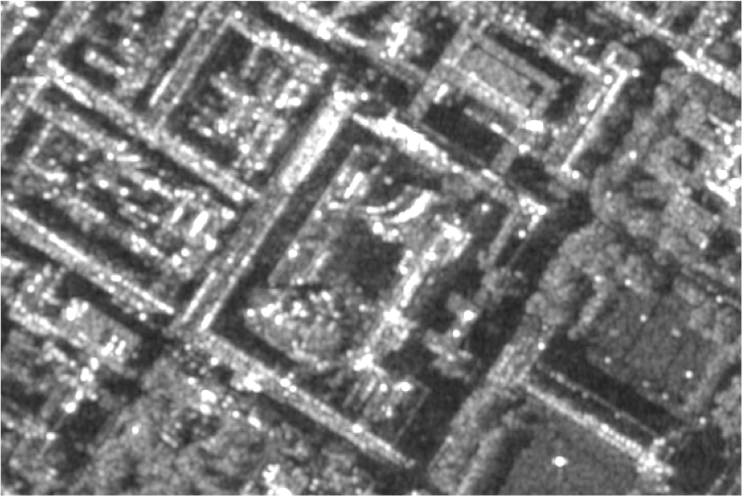
\includegraphics[width=0.9\linewidth]{../figures/franceschetti_2007_munich_sar}
	\caption{An actual SAR image of a portion of Munich}
	\label{fig:franceschetti_2007_munich_sar}
\end{subfigure}%
\begin{subfigure}{.5\textwidth}
	\centering
	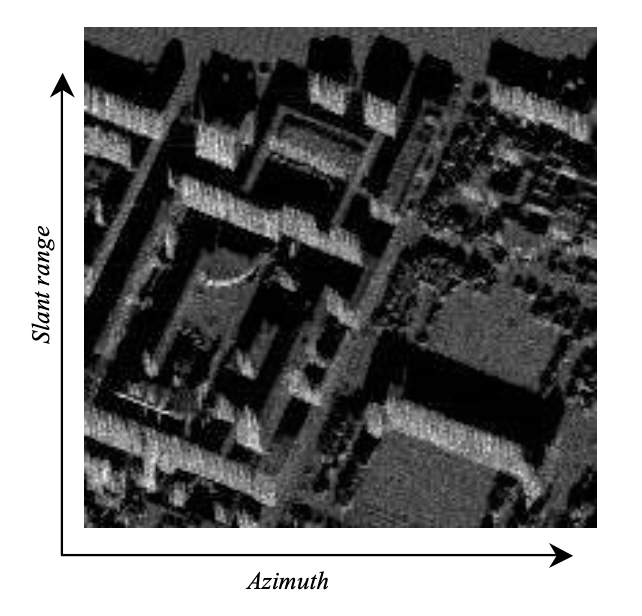
\includegraphics[width=0.9\linewidth]{../figures/franceschetti_2007_munich_sim}	
	\caption{A simulated SAR image of the same area}
	\label{fig:franceschetti_2007_munich_sim}
\end{subfigure}
\caption{A comparison between an actual SAR image and simulated SAR image of the Technische Universität and Alte Pinakothek from \cite{franceschettiSimulationToolsInterpretation2007}}
\label{fig:franceschetti_2007_munich}
	
\end{figure}

A similar approach building on the previously mentioned work is presented by Zheng \textit{et al.} \cite{zhengSimulationMethodSAR2008} which uses the scattering model in order to accurately simulate a SAR scene. This is achieved by making the assumption that the scene is made up of vertical buildings distributed on a rough dielectric terrain. This also discusses the computation of scattering coefficients under different conditions. As with the previous approach (and the following raw SAR approach) the Kirchhoff approach is used in this case.
\par
A similar approach to robust SAR simulation is described in Dellière \textit{et al.} 2007 \cite{delliereSARMeasurementSimulation2007}, which uses an electromagnetic approach closely following Maxwell's equations to create a finite-difference time domain method of simulation, which differs from \cite{franceschettiSARRawSignal2003} as that instead manipulates the signal in the frequency domain in order to create the raw SAR signal. This system has similar drawbacks to Franceschetti's approach with regards to computation complexity and time required, but is even more computationally complex, due to its ability to handle dispersive materials as well as phase changes. This approach could be of some interest for creating an incredibly robust simulator due to the advances in computing performance between the publication date and today. \par
\subsubsection{Graphical SAR Simulation}
There are two methods that are less complex computationally for simulating the image achieved by SAR. These both arise from graphics manipulation and more specifically 3 dimensional modelling. These are rasterisation and ray tracing. Rasterisation is the process of taking a 3 dimensional area and creating a 2 dimensional image using some sort of image transformation based on the location of the camera to the object in the 3D area. Ray tracing follows a similar process to light, just in reverse. It sends beams out from the camera in all directions that the camera can see and simulates them reflecting off of objects until they hit a source of illumination. Using this the rendering engine can determine if an object is illuminated or not and adjust appropriately. These two approaches have both been used in the past for simulation of SAR images. Rasterisation was used by Balz 2006 \cite{balzRealtimeSARSimulation2006} and ray tracing was explored by Auer \textit{et al.} 2008 \cite{auerRayTracingSimulating2008} and Mametsa \textit{et al.} 2002 \cite{mametsaImagingRadarSimulation2002}. This second paper was used in Hammer \textit{et al.} \cite{hammerComparisonSARSimulation2008} along with Balz 2006 to compare the relative merits of these two approaches. Ultimately the advantages of Balz's approach as detailed in \cite{balzImprovedRealTimeSAR2006} and \cite{balzRealtimeSARSimulation2006} is that the simulator is real-time so can be used to determine optimal azimuthal directions when recording a SAR image using a physical airborne platform. This form of simulation however doesn't take into account the contributions of higher order reflections so if it is being used for a demonstration tool, the images produced are less representative of an actual SAR image. This also means that corners aren't visible in the image, meaning that this form of simulation can't be used to test feature extraction algorithms. The two ray tracing simulators tested within \cite{hammerComparisonSARSimulation2008} can simulate these higher-order contributions meaning they can be used to test feature extraction algorithms, however due to the computationally intensive nature of ray tracing these can't be simulated in real time, so this form of simulation is less useful for planning purposes. \par
\begin{figure}
\centering
\begin{subfigure}{.5\textwidth}
	\centering
	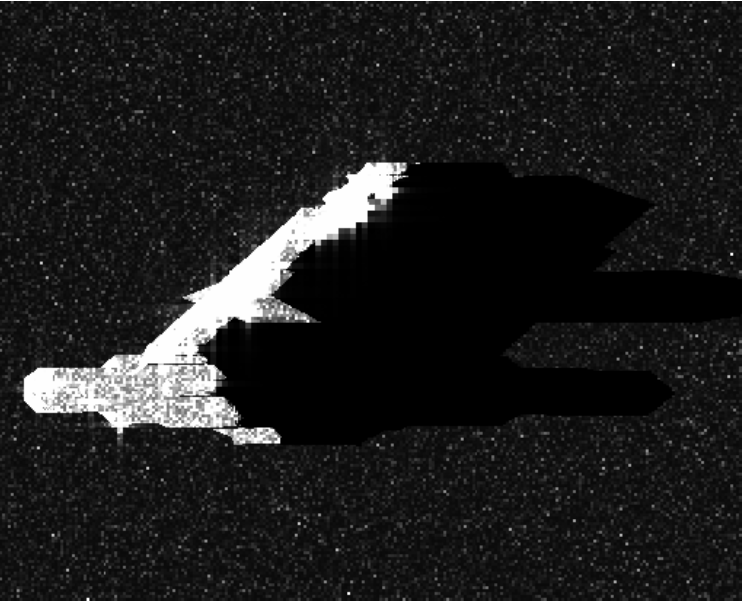
\includegraphics[width=0.9\linewidth]{../figures/balz_2006_stiftskirche}
	\caption{0.3m resolution simulation of the Stiftskirche in Stuttgart}
	\label{fig:balz_2006_stiftskirche}
\end{subfigure}%
\begin{subfigure}{.5\textwidth}
	\centering
	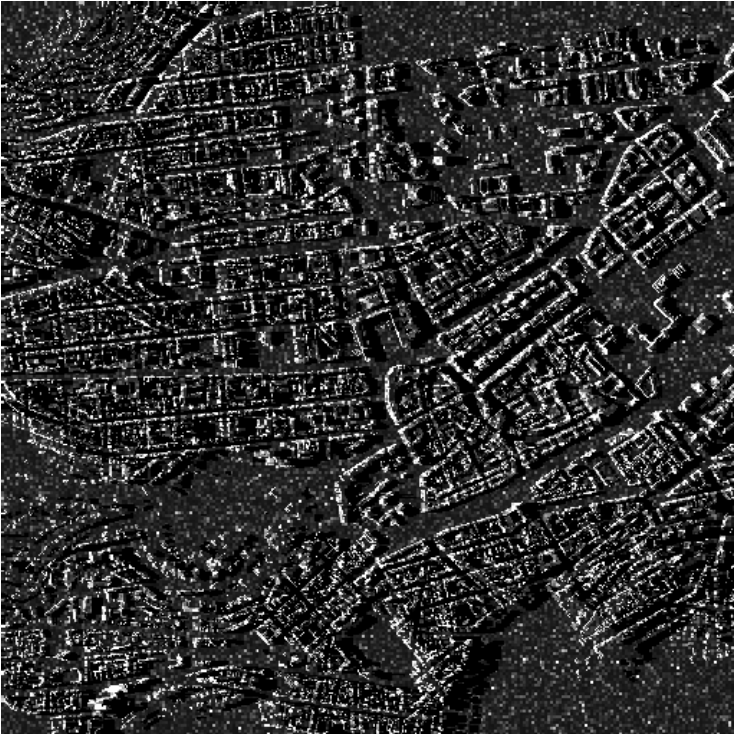
\includegraphics[width=0.9\linewidth]{../figures/balz_2006_stuttgart}	
	\caption{5m resolution simulation of Stuttgart}
	\label{fig:balz_2006_stuttgart}
\end{subfigure}
\caption{Results from Balz 2006 \cite{balzImprovedRealTimeSAR2006} using rasterisation techniques}
\label{fig:balz_2006_images}
	
\end{figure}

\begin{figure}
\centering
\begin{subfigure}{.5\textwidth}
	\centering
	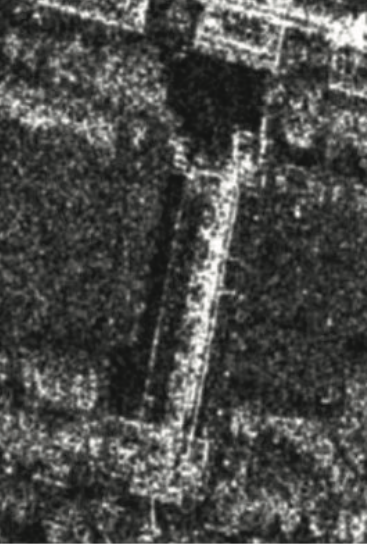
\includegraphics[width=0.9\linewidth]{../figures/auer_2008_terrasar_ref}
	\caption{A reference spotlight image of the Alta Pinakothek}
	\label{fig:auer_2008_ref}
\end{subfigure}%
\begin{subfigure}{.5\textwidth}
	\centering
	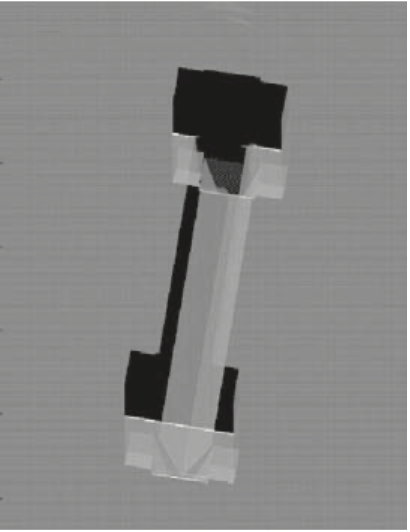
\includegraphics[width=0.9\linewidth]{../figures/auer_2008_all_reflections}	
	\caption{A simulated SAR image using ray tracing of the Alta Pinakothek}
	\label{fig:auer_2008_all}
\end{subfigure}
\caption{Simulated SAR using ray tracing from Auer \textit{et al.} 2008 \cite{auerRayTracingSimulating2008}}
\label{fig:auer_2008_ray_tracing}
	
\end{figure}


All of the forms of simulation presented here so far are only as good as the models used, as generally the modelled buildings are assumed to be made of one material with a fixed dielectric constant, while the modelled ground is made of a different material. In \cite{hammerComparisonSARSimulation2008}, the buildings modelled are created entirely of stone, with a grass ground. In real life however this becomes more complicated as buildings do tend to be made up of multiple materials, and often in urban areas the ground is made up of a material with a similar dielectric constant to the buildings. This also doesn't include any forms of dispersive materials such as metal. It is unclear whether any of the simulators covered in \cite{hammerComparisonSARSimulation2008} can simulate these sorts of materials accurately, which is something that should be taken to account in the future. \par
Yet another method similar to the image processing approaches is presented by Lu \textit{et al.} \cite{luGPUBasedRealtime2009} and uses methods most commonly used by video games. In this case the raw mathematic SAR simulation is not carried out, similar to \cite{balzHybridGPUBasedSingle2009} and \cite{auerRayTracingSimulating2008} and uses an orthogonal projection to cast the 3D model to a 2D image based on the slant range of the camera. This again has the potential of improving the performance of image generation in incredibly complicated scenes such as city centres.
\par 
\subsubsection{Hybrid Method and Other Papers of Note}
Chen \textit{et al.} 2011 \cite{chenRadarImagingSimulation2011} proposes a hybrid method of simulating these images using analytical models. In this approach, the contributions provided by backscattering are shown using an electromagnetic analytical model ultimately based on that described by \cite{franceschettiSARRawSignal2003}, and the object position vectors are given by a geometric model using ray tracing. In this paper the analysis is mostly focused on cylindrical or cylinder-like buildings, with some analysis devoted to flat-roof buildings as well. This approach has a potential to be more accurate than the ray tracing models proposed previously due to the electromagnetic models involved, but also be less computationally complex than the more canonical SAR image simulators. 
\par
Xu and Jin 2006 \cite{xuImagingSimulationPolarimetric2006} is a paper that is not immediately relevant to this situation due to it modelling natural environments for SAR simulation however this is potentially interesting and relevant due to the variety of materials present in urban environments to be modelled. This is an algorithm that can deal with randomly and heterogeneously distributed objects within an image with varying dielectric constants and can deal with them in a reasonable length of time. This is something that is worth exploring if there is time in the future as it would add robustness to the system as a whole. 






